\documentclass{article}

\usepackage{fullpage}
\usepackage{graphicx}
\usepackage{subcaption}

\begin{document}

\section{Introduction}

We are trying to understand the cost of uvm hmm on a range of
scenario. We'll look at a simple application to have a sense of the
impact of arithmetic intensity.

The assumption that we are trying to confirm is that essentially UVM
and HMM give you normal processing but at lower interconnect speed.

\section{Polynomial Expansion}

\subsection{Problem}

You have a bunch of points $x_0, \dots, x_n$. For each you want to compute a polynomial $P(x) = \sum_{i=0}^d c_i x^i$.

Note the calculation is in $\Theta(n(d+1))$, it moves $\Theta(n+d)$ memory and do $\Theta(n(d+1))$ flops.

\subsection{cpu implementation}

two implems.

one sequential

one openmp

\subsection{cuda implementation}

Basic implementation is pretty much what you think it is. Init on CPU,
alloc array for x and coefficients on the gpu. Cuda memcpy the data
over. A cuda kernel, one cuda thread per entry in the array who does
$d+1$ muls and adds. Memcopy results back.

The pinned implementation is the same. But the CPU memory is allocated
in page-locked memory. So the cudamemcopy is faster.

The stream implementation aims to get communiucation comptation
overlap. It splits the calculation in a number of streams. Each stream
processes many chunks of a fixed size. The stream does memcopy data
in, launch kernel, memcpy data back.

The UVM implementation allocs the memory with cudamallocmanaged which
makes the memory managed by the uvm driver. Becasue we get gpu side
paging, there is no memcopy, the kernel work straight out of the memory.

The basic and pinned implementations are naturally limited to GPU
memory. While the stream and UVM implementation can process more data
than the GPU can hold.

\section{Modeling}

\subsection{A steady state model}

The problem is essentially 3 phased. move data in, do the calculation,
move data out. The move data in and out are happening on the
interconnect (pci-e or nvlink). The calculation itself has two main
components, how much data you need to move (roughly $\Theta(n)$) and
how much computation you do $\Theta(nd)$. The runtime of the kernel
itself will be defined by the bottleneck which could be either data or
flops: $max(\frac{2n(d+1)}{gpuflops},
\frac{2n*sizefp32}{gpumembw})$. Moving data in and out of the gpu is
given by the time to transfer over the interconnect
$\frac{(n+d+1)sizefp32}{interconnectBW}$

Depending on the implementation you get communication/computation
overlap or not. If you do get communication/computation overlap, the
runtime is given by the maximum between communication time and computation time:

$max(max(\frac{2n(d+1)}{gpuflops}, \frac{2n*sizefp32}{gpumembw}),\frac{(n+d+1)sizefp32}{interconnectBW})$

But if there is no overlap then the two happen one after the other and
the application time is

$max(\frac{2n(d+1)}{gpuflops}, \frac{2n*sizefp32}{gpumembw}) +
\frac{(n+d+1)sizefp32}{interconnectBW}$

\subsection{Modeling limitation}

That model is quite flawed. It assumes that calculation enters steady
states and so that you actually do reach a bandwidth style bottleneck
on one of the ressource.  It assumes there is no complex interaction
in the system that cause chain of event delays in the calculation.

That assumption is probably reasonnable at large scale, the
experimental results will confirm that.

At smaller scale (smaller $n$ values) than there should be a lot more
latency effects.

\subsection{Calibrating}

To use the models we'll to calibrate the flops and banwidth ratings.

We'll use actual measurement from the code to calibrate. We will
calibrate flops using a gpu only measurement for a run with a large
degree and derive flops from that. For gpubw, we take a measurement
with degree 0 and large $n$. And for interconnect measurment we take a
total overlapped execution with degree 0 and large $n$.

\section{Experiments}

We ran on a bunch of different machines. Here are some results on
hopper 1 and hopper 2.

\begin{figure}[htbp]
  \centering
  \begin{subfigure}[b]{0.45\textwidth}
    \centering
    \includegraphics[width=\textwidth,page=5]{analysis-cci-hopper1.pdf}
    \caption{Hopper1, n=16B (non-oversubscribed)}
  \end{subfigure}
  \begin{subfigure}[b]{0.45\textwidth}
    \centering
    \includegraphics[width=\textwidth,page=5]{analysis-cci-hopper2.pdf}
    \caption{Hopper2, n=16B (non-oversubscribed)}
  \end{subfigure}

  \begin{subfigure}[b]{0.45\textwidth}
    \centering
    \includegraphics[width=\textwidth,page=7]{analysis-cci-hopper1.pdf}
    \caption{Hopper1, n=64B (oversubscribed)}
  \end{subfigure}
  \begin{subfigure}[b]{0.45\textwidth}
    \centering
    \includegraphics[width=\textwidth,page=6]{analysis-cci-hopper2.pdf}
    \caption{Hopper2, n=64B (oversubscribed)}
  \end{subfigure}

  \begin{subfigure}[b]{0.45\textwidth}
    \centering
    \includegraphics[width=\textwidth,page=13]{analysis-cci-hopper1.pdf}
    \caption{Hopper1, d=1024}
  \end{subfigure}
  \begin{subfigure}[b]{0.45\textwidth}
    \centering
    \includegraphics[width=\textwidth,page=12]{analysis-cci-hopper2.pdf}
    \caption{Hopper2, d=1024}
  \end{subfigure}

  \label{fig:perf-hopper}
  \caption{perf results on Hopper GPUs, hopper1 is x86 cpu side; hopper2 is grace.}
\end{figure}

Figure~\label{fig:perf-hopper} presents results on hopper gpus with an
grace/nvlink configuration and a x86/pcie configuration. We present
all performance in flops for normalization. We present both the
performance a prediction of that performance based on the model
described above.

Some observations:

The models are fairly accurate. Rarely more than 15\% off. They are
only off on really small arrays; which make sense the size are
probably not high enough to saturate any part of the system so you get
latency effects and a steady state model becomes wrong.

The fact that the model is accurate means that the difference in
performance between \texttt{gpu\_uvm} and \texttt{gpu\_stream} is
mostly explained by the difference in effective interconnect bandwidth
experienced by UVM.

With densification of arithmetic intensity, the difference between UVM
and stream decreases and it eventually decreases to essentially no
difference at a degree of 4098; so at 8192 flops per FP32 float; or at
2048 flops per byte

You can measure the difference in arithmetic intensity for different
memory management model. While stream saturates gpu flops at roughly
degree 256, you need roughly 4098 to saturate with UVM.

You can see that at small $n$ values, the model is less accurate. This
is most likely an effect of

What's going on with pageable memory speed? No idea.

It is interesting that we see that the peak flop performance is about
the same between hopper1 and hopper 2. But hopper 2 show more
performance in its interconnect, which we expect since nvlink.

We also see that there is no real performance cost to
oversubscription, the calculation is interconnect bound but the
bandwidth is used just as effectively in undersubscribed and over
subscribed cases.

\end{document}
